\documentclass[12pt,a4paper]{article}
\usepackage[utf8]{inputenc}
\usepackage[T1]{fontenc}
\usepackage[margin=2.5cm,headheight=16pt,headsep=18pt]{geometry}
\usepackage{graphicx}
\usepackage{fancyhdr}
\usepackage{booktabs}
\usepackage{tabularx}
\usepackage{amsmath}
\usepackage{tikz}
\usepackage[hidelinks]{hyperref}
\graphicspath{{docs/}{./}}

\renewcommand{\contentsname}{Daftar Isi}
\renewcommand{\appendixname}{Lampiran}
\renewcommand{\tablename}{Tabel}
\renewcommand{\figurename}{Gambar}
\setcounter{tocdepth}{3}
\setlength{\parindent}{1.5em}
\setlength{\parskip}{0pt}

\pagestyle{fancy}
\fancyhf{}
\fancyhead[L]{IF3170 -- Inteligensi Artifisial}
\fancyhead[R]{\thepage}
\renewcommand{\headrulewidth}{0.4pt}
\renewcommand{\footrulewidth}{0pt}

% Kompilasi dari root repositori (jalankan dua kali agar daftar isi terbarui):
% pdflatex -output-directory=docs docs/laporan.tex
% Bab 1 dan 2 sudah diisi; rincian implementasi dan hasil eksperimen menyusul.
\begin{document}

\hypersetup{pageanchor=false}
\begin{titlepage}
    \centering
    {\Huge\bfseries Laporan Tugas Besar 1\par}
    \vspace{0.5cm}
    {\LARGE\scshape IF3170 Inteligensi Artifisial\par}
    \vspace{0.3cm}
    {\Large\scshape Optimasi Pengisian Paket pada Truk Peti Kemas\par}
    \vspace{0.2cm}
    {\Large\scshape dengan Algoritma Local Search\par}
    \vspace{0.3cm}
    {\Large\scshape Tahun Akademik 2026--2027\par}
    \vfill
    % Logo dari situs resmi ITB:
    % https://itb.ac.id/assets/images/Logo%20ITB_COLOR_2026%404x.png
    
\includegraphics[width=7.5cm,keepaspectratio]{logo-itb.png}\par
    \vfill
    {\large\bfseries Disusun oleh:\par}
    \vspace{0.3cm}
    {\large Kelompok 37\par}
    \vspace{0.3cm}
    {\large Samuelson Dharmawan Tanuraharja -- 13524001\par}
    {\large Nicholas Wise Saragih Sumbayak -- 13524037\par}
    {\large Neswa Eka Anggara -- 13524136\par}
    \vfill
    {\large\scshape Laboratorium Inteligensi Artifisial\par}
    {\large\scshape Program Studi Teknik Informatika\par}
    {\large\scshape Sekolah Teknik Elektro dan Informatika\par}
    {\large\scshape Institut Teknologi Bandung\par}
\end{titlepage}

\pagenumbering{arabic}
\hypersetup{pageanchor=true}
\tableofcontents
\clearpage

\section{Pendahuluan}
\subsection{Latar Belakang}
Mejiro Express, usaha logistik darat dalam studi kasus tugas besar ini, perlu menentukan paket yang akan dimuat ke dalam peti kemas truk beserta susunannya. Special Week sebagai pengemudi membutuhkan keputusan yang cepat, sedangkan paket memiliki ukuran, nilai, berat, dan sifat kerapuhan yang berbeda. Memasukkan seluruh paket belum tentu mungkin: ruang dan kapasitas angkut terbatas, paket tidak boleh saling menembus, serta susunannya harus ditopang dengan benar. Oleh karena itu, persoalannya mencakup pemilihan paket sekaligus pengaturan ruang tiga dimensi \cite{spesifikasi}.

Jumlah kombinasi pilihan paket, posisi, dan orientasi bertambah ketika jumlah paket meningkat. Menelusuri seluruh konfigurasi secara langsung menjadi kurang praktis. Tugas besar ini menggunakan \textit{local search} untuk memperbaiki konfigurasi secara bertahap dan membandingkan kualitas hasil dari beberapa metode pencarian \cite{spesifikasi,slide-local-search}.

\subsection{Rumusan Persoalan dan Tujuan}
Masukan persoalan berupa sejumlah paket berbentuk balok atau kubus dan peti kemas dengan dimensi serta kapasitas angkut tertentu. Untuk setiap paket, perlu diputuskan apakah paket dimuat; jika dimuat, perlu ditentukan posisi dan orientasinya. Keluaran yang dicari ialah konfigurasi sah dengan jumlah nilai paket termuat setinggi mungkin. Paket yang tidak dipilih tetap tercatat sebagai paket di luar peti kemas \cite{spesifikasi}.

Tujuan pekerjaan ini adalah membangun dan mengevaluasi pencarian konfigurasi menggunakan sedikitnya satu varian \textit{hill climbing}, \textit{simulated annealing}, dan \textit{genetic algorithm}. Perbandingan dilakukan melalui nilai solusi, perkembangan nilai selama iterasi, durasi pencarian, dan pengulangan percobaan sesuai ketentuan tugas \cite{spesifikasi}.

\subsection{Ruang Lingkup Persoalan}
Dimensi paket dan peti kemas dinyatakan pada tiga sumbu ruang; posisi paket memakai koordinat bilangan bulat. Setiap paket dapat memiliki orientasi hasil rotasi siku-siku terhadap sumbu ruang. Konfigurasi dianggap sah apabila paket termuat seluruhnya di dalam peti kemas, tidak bertumpang tindih, tidak melayang, tidak bertumpu pada paket rapuh, dan jumlah beratnya tidak melampaui kapasitas angkut. Suatu paket boleh sepenuhnya berada di luar peti kemas \cite{spesifikasi}.

\begin{figure}[htbp]
    \centering
    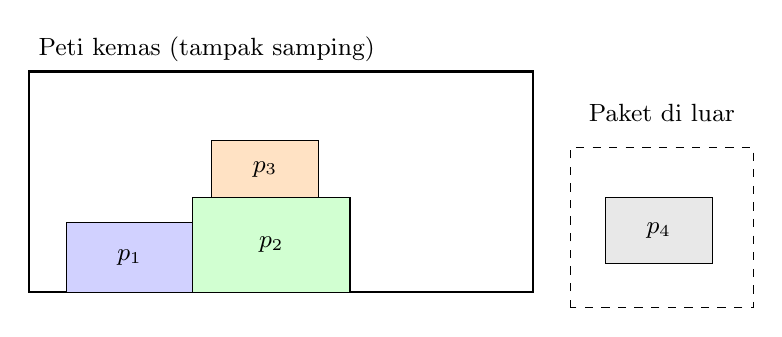
\begin{tikzpicture}[scale=0.8, every node/.style={font=\small}]
        \draw[thick] (0,0) rectangle (8,3.5);
        \node[anchor=south west] at (0,3.5) {Peti kemas (tampak samping)};
        \filldraw[fill=blue!18] (0.6,0) rectangle (2.6,1.1);
        \node at (1.6,0.55) {$p_1$};
        \filldraw[fill=green!18] (2.6,0) rectangle (5.1,1.5);
        \node at (3.85,0.75) {$p_2$};
        \filldraw[fill=orange!23] (2.9,1.5) rectangle (4.6,2.4);
        \node at (3.75,1.95) {$p_3$};
        \draw[dashed] (8.6,-0.25) rectangle (11.5,2.3);
        \node[align=center] at (10.05,2.85) {Paket di luar};
        \filldraw[fill=gray!18] (9.15,0.45) rectangle (10.85,1.5);
        \node at (10,0.98) {$p_4$};
    \end{tikzpicture}
    \caption{Ilustrasi konseptual paket termuat dan paket di luar peti kemas. Susunan sebenarnya ditentukan dalam tiga dimensi.}
    \label{fig:ilustrasi-pemuatan}
\end{figure}

\clearpage
\section{Dasar Teori}
\subsection{Optimisasi Kombinatorial dan \textit{Local Search}}
Pada masalah optimisasi, sebuah keadaan mewakili satu kandidat jawaban dan fungsi objektif memberi nilai pada kandidat tersebut. Dalam persoalan pemuatan, yang dinilai adalah konfigurasi akhir paket, bukan urutan langkah yang menghasilkan konfigurasi itu. Karena itu, pendekatan \textit{local search} sesuai: pencarian dimulai dari konfigurasi awal, lalu mengunjungi konfigurasi tetangga untuk mencari nilai yang lebih baik \cite[Bag.~4.1]{russell-norvig}, \cite{slide-local-search}.

Misalkan $P$ adalah himpunan paket, $v_i$ nilai paket $i$, dan $I_i(s)$ bernilai satu jika paket $i$ termuat pada keadaan $s$ serta nol jika tidak. Fungsi objektif utama dapat ditulis sebagai
\begin{equation}
    \max_{s\in\mathcal{F}} f(s), \qquad
    f(s)=\sum_{i\in P} v_i I_i(s),
    \label{eq:objektif-utama}
\end{equation}
dengan $\mathcal{F}$ himpunan konfigurasi yang memenuhi seluruh batasan. Nilai yang tinggi tidak membenarkan susunan yang tidak sah; batasan menentukan apakah suatu kandidat termasuk $\mathcal{F}$ \cite{spesifikasi}. Jika lebih dari satu truk digunakan, indikator $I_i(s)$ tetap menyatakan apakah paket termuat pada salah satu truk, sehingga nilai paket dihitung sekali.

\subsection{Keadaan, Tetangga, dan Lanskap Pencarian}
Keadaan atau \textit{state} adalah deskripsi lengkap satu konfigurasi, termasuk paket yang termuat dan yang berada di luar. Tetangga ialah konfigurasi yang diperoleh melalui perubahan terbatas terhadap keadaan sekarang. Spesifikasi memperbolehkan penukaran dua paket, pemindahan sebuah paket ke koordinat lain, dan rotasi paket sebesar $90^\circ$ terhadap sumbu $x$, $y$, atau $z$. Keadaan awal dibangkitkan secara acak \cite{spesifikasi}.

Jika setiap keadaan dipandang sebagai titik dan nilainya sebagai ketinggian, pencarian membentuk suatu lanskap. Puncak lokal memiliki nilai setidaknya sebesar tetangga di sekitarnya, tetapi mungkin masih lebih rendah daripada puncak global. Dataran bernilai sama atau \textit{plateau} juga dapat membuat pencarian sulit bergerak. Bentuk lanskap bergantung pada definisi tetangga dan batasan sah, sehingga pilihan operasi perubahan ikut memengaruhi hasil pencarian \cite[Bag.~4.1]{russell-norvig}, \cite{slide-local-search}.

\subsection{\textit{Hill Climbing}}
\textit{Hill climbing} berpindah menuju tetangga yang nilainya lebih tinggi. Pada varian \textit{steepest-ascent}, seluruh tetangga yang dipertimbangkan dievaluasi dan dipilih yang terbaik. Pada varian stokastik, kandidat tetangga diperiksa secara acak dan perpindahan diterima jika memperbaiki nilai. Keduanya dapat berhenti pada puncak lokal karena tidak menerima penurunan nilai \cite[Bag.~4.1]{russell-norvig}, \cite{slide-local-search}.

Varian \textit{sideways move} mengizinkan sejumlah perpindahan menuju tetangga dengan nilai sama agar pencarian dapat melintasi \textit{plateau}; batas jumlah langkah tersebut mencegah perpindahan tanpa akhir. \textit{Random-restart hill climbing} mengulangi pencarian dari keadaan awal acak yang berbeda untuk menjelajahi daerah lain pada lanskap. Dalam pemuatan paket, kedua pendekatan ini berguna ketika beberapa pertukaran atau perpindahan tidak langsung menaikkan total nilai paket termuat \cite[Bag.~4.1]{russell-norvig}, \cite{slide-local-search}.

\subsection{\textit{Simulated Annealing}}
\textit{Simulated annealing} menerima tetangga yang lebih baik, tetapi kadang juga menerima tetangga yang lebih buruk untuk keluar dari puncak lokal. Untuk perubahan nilai $\Delta f=f(s')-f(s)<0$ pada temperatur $T>0$, peluang menerima tetangga $s'$ adalah
\begin{equation}
    \Pr(\text{terima }s')=\exp\!\left(\frac{\Delta f}{T}\right).
    \label{eq:annealing}
\end{equation}
Temperatur yang lebih tinggi membuat penurunan nilai lebih mungkin diterima; ketika temperatur turun, pencarian menjadi semakin selektif. Jadwal penurunan temperatur dan batas iterasi memengaruhi keseimbangan antara menjelajahi konfigurasi baru dan mempertahankan konfigurasi bernilai tinggi \cite[Bag.~4.1]{russell-norvig}, \cite{slide-local-search}. Dalam persoalan ini, langkah yang diterima tetap harus memenuhi batasan fisik pemuatan.

\subsection{\textit{Genetic Algorithm}}
\textit{Genetic algorithm} mengolah sekumpulan keadaan sekaligus sebagai populasi. Setiap individu diberi nilai \textit{fitness}, kemudian pemilihan induk, \textit{crossover}, dan mutasi menghasilkan generasi berikutnya. Pemilihan cenderung mengutamakan individu bernilai tinggi, sedangkan \textit{crossover} menggabungkan bagian dari dua konfigurasi dan mutasi menambah keragaman pencarian \cite[Bag.~4.1]{russell-norvig}, \cite{slide-local-search}.

Pada pemuatan paket, satu individu menggambarkan susunan lengkap. Penggabungan dan mutasi dapat menghasilkan kandidat yang melanggar batas ruang atau aturan tumpukan; karena itu, penilaian individu harus dikaitkan dengan pemeriksaan kelayakan. Ukuran populasi dan jumlah generasi menentukan banyaknya kandidat yang dijelajahi serta biaya komputasinya. Rincian representasi individu, operator yang dipakai, dan penanganan kandidat tidak sah menjadi bagian pembahasan implementasi pada Bab~3.

\clearpage
\section{Pembahasan}
\subsection{Implementasi Algoritma \textit{Local Search}}
\subsubsection{Representasi State dan Inisialisasi}
\subsubsection{Pembangkitan Tetangga}
% Siapkan deskripsi fungsi/kelas beserta source code yang relevan di tiap subbagian.
\subsubsection{Hill Climbing}
\subsubsection{Simulated Annealing}
\subsubsection{Genetic Algorithm}
\subsubsection{Validasi Batasan dan Evaluasi Fungsi Objektif}

\clearpage
\subsection{Rancangan Eksperimen}
\subsubsection{Data Uji dan Lingkungan Eksperimen}
\subsubsection{Konfigurasi Parameter dan Pengulangan Eksperimen}

\clearpage
\subsection{Hasil Eksperimen dan Visualisasi Program}
\subsubsection{Hill Climbing}
\subsubsection{Simulated Annealing}
\subsubsection{Genetic Algorithm}
\subsubsection{Visualisasi State Awal dan State Akhir}

\subsection{Analisis Eksperimen}
\subsubsection{Perbandingan Kualitas Solusi}
\subsubsection{Perbandingan Durasi Pencarian}
\subsubsection{Konsistensi Hasil Eksperimen}
\subsubsection{Pengaruh Parameter Genetic Algorithm}

\clearpage
\section{Kesimpulan dan Saran}
\subsection{Kesimpulan}
\subsection{Saran}

\section{Pembagian Tugas Tiap Anggota Kelompok}
\begin{table}[ht]
    \centering
    \renewcommand{\arraystretch}{1.5}
    \begin{tabularx}{\textwidth}{@{}p{7cm}lX@{}}
        \toprule
        \textbf{Nama Lengkap} & \textbf{NIM} & \textbf{Tugas/Kontribusi} \\
        \midrule
        Samuelson Dharmawan Tanuraharja & 13524001 & \\
        Nicholas Wise Saragih Sumbayak & 13524037 & \\
        Neswa Eka Anggara & 13524136 & \\
        \bottomrule
    \end{tabularx}
    \caption{Pembagian tugas anggota kelompok}
\end{table}

\section*{Daftar Pustaka}
\addcontentsline{toc}{section}{Daftar Pustaka}
\begin{thebibliography}{9}
\bibitem{spesifikasi}
Tim Asisten Laboratorium Inteligensi Artifisial, \emph{Spesifikasi Tugas Besar 1 IF3170 Inteligensi Artifisial 2026/2027}, versi 1.4, Institut Teknologi Bandung, 24 September 2026.

\bibitem{russell-norvig}
S. J. Russell dan P. Norvig, \emph{Artificial Intelligence: A Modern Approach}, edisi ke-4, Pearson, 2021, Bab 4.

\bibitem{slide-local-search}
Tim Pengajar IF3170 Inteligensi Artifisial, \emph{Beyond Classical Search}, bahan presentasi kuliah, Institut Teknologi Bandung, Semester I 2026/2027.
\end{thebibliography}

\appendix
\section{Form Penggunaan Generative AI}
% Lampirkan formulir resmi dari halaman 19 Panduan AI ITB.
% Belum diisi: setiap anggota harus mencatat penggunaan AI yang sebenarnya.
% Penggunaan AI dalam penyusunan kerangka laporan ini juga perlu dicatat.
% Jangan membuat pernyataan, persetujuan, atau tanda tangan atas nama anggota.

\section{Lampiran Lainnya (Bila Ada)}

\end{document}
